\documentclass[a4paper, 10pt]{article}
%\usepackage{fontspec}
%\setmainfont{Lato}
\usepackage{pgf}
\usepackage{eurosym}
\usepackage{graphicx}
\usepackage{wasysym}
\usepackage{hyperref}
\usepackage{listings}
\usepackage{pxfonts}
\usepackage{verbatim}
\usepackage{color}
\usepackage{xcolor}
\usepackage{wrapfig}
\usepackage{enumitem}
\usepackage{booktabs}
\usepackage{gensymb}
\usepackage{tabularx}
\usepackage{currfile}

\hypersetup{
    bookmarks=true,         % show bookmarks bar?
    unicode=true,          % non-Latin characters in Acrobat’s bookmarks
    pdftoolbar=true,        % show Acrobat’s toolbar?
    pdfmenubar=true,        % show Acrobat’s menu?
    pdffitwindow=true,     % window fit to page when opened
    pdftitle={Assessments},    % title
    pdfauthor={Paul Vesey},     % author
    pdfsubject={Advanced Graphics Assignment },   % subject of the document
    pdfcreator={},   % creator of the document
    pdfproducer={xelatex}, % producer of the document
    pdfkeywords={'Graphics' }, % list of keywords
    pdfnewwindow=true,      % links in new PDF window
    colorlinks=true,       % false: boxed links; true: colored links
    linkcolor=violet,          % color of internal links (change box color with linkbordercolor)
    citecolor=magenta,        % color of links to bibliography
    filecolor=red,      % color of file links
    urlcolor=blue           % color of external links
}

\setlength\parindent{0pt}
\begin{document}

\lstset{language=HTML,
				basicstyle=\small,
				breaklines=true,
        numbers=left,
        numberstyle=\tiny,
        showstringspaces=false,
        aboveskip=-20pt,
        frame=leftline
        }
				
\begin{table}%
	\begin{minipage}{0.4\textwidth}%
			
\includegraphics[width=1\textwidth]{./img/LITlogo.jpg}
	\end{minipage}
	\qquad
	\centering
	\parbox{0.4\textwidth}{
		\begin{large}			
			\begin{tabular}{| r | l |} \hline
				Subject: & \textbf{Advanced Graphics}\\
								 & \textbf{\& Visualisation}\\
				Course: & \textbf{Interior Design Y3}\\
				Session: & \textbf{Autumn 2020}\\
				Lecturer: & \textbf{Paul Vesey \footnotesize{BEng, MIE, HDip}}\\
				Filename: & \footnotesize{\currfilename}\\
				\hline
			\end{tabular}
		\end{large}			
	}
\end{table}
\vspace{0.25cm}	
	
\begin{flushleft}
\Large\textbf{Assignment 1 (5\%) - 3D Assets }\\
\end{flushleft}

This assignment involves collecting high quality assets and rendering them for display.  In total you are to download and clean-up 10 models from one of the categories below.  At least two models must be 'iconic' examples of the category, such as the 1948 Isamu Noguchi coffee table.  Your submission will be used to create and expand a library of furniture that we will use during the year.

\begin{enumerate}
	\item Chair.
	\item Sofa Suite
	\item Table
	\item Bed
	\item Desk
	\item Lamp (Table, Floor, Wall)
	\item Wardrobe
	\item Picture Frames
	\item Shelf Units
	\item Rug
	\item Bathroom Suite x 3: (Bath, Toilet, Sink)
\end{enumerate}

For each item in your submission you must submit the following:

\begin{enumerate}
	\item Clean .max file of the item, correctly scaled with minimal materials included.
	\item Studio .max file similar to the examples shown.
	\item 1028 x 764 beauty render in .jpg format
	\item 1028 x 764 shaded wire-frame render in .jpg format
\end{enumerate}

You are advised to create the studio .max file first and create the necessary renders.  Once the renders are complete, simply delete the background, lights and camera, and Save-As a new file. \\

Example images are provided below, and the max files used are available on GitHub.\\

Final submission is to be a zip file containing separate folders for each furniture item.\\

\vspace{1cm}

\begin{figure}[hb]
	\centering
		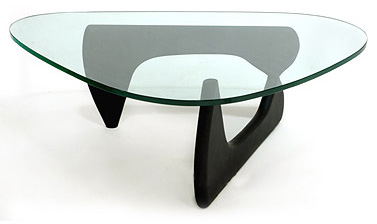
\includegraphics[width=10cm]{img/noguchi-1948.jpg}
		\caption{Isamu Noguchi, Coffee Table, 1948}
	\label{fig:noguchi-1948}
\end{figure}


\begin{figure}[hb]
	\centering
		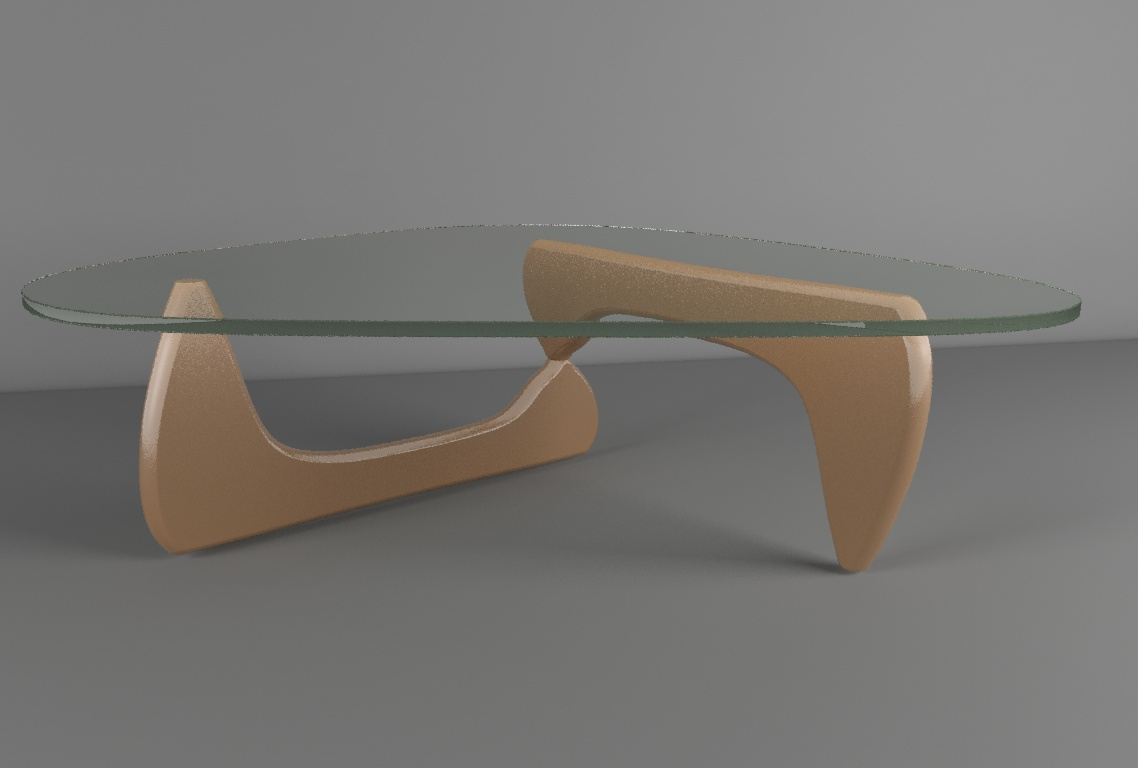
\includegraphics[width=10cm]{img/CoffeTableBeauty.jpg}
		\caption{Mental Ray Render, Beauty Pass}
	\label{fig:noguchi-1948}
\end{figure}

\begin{figure}[hb]
	\centering
		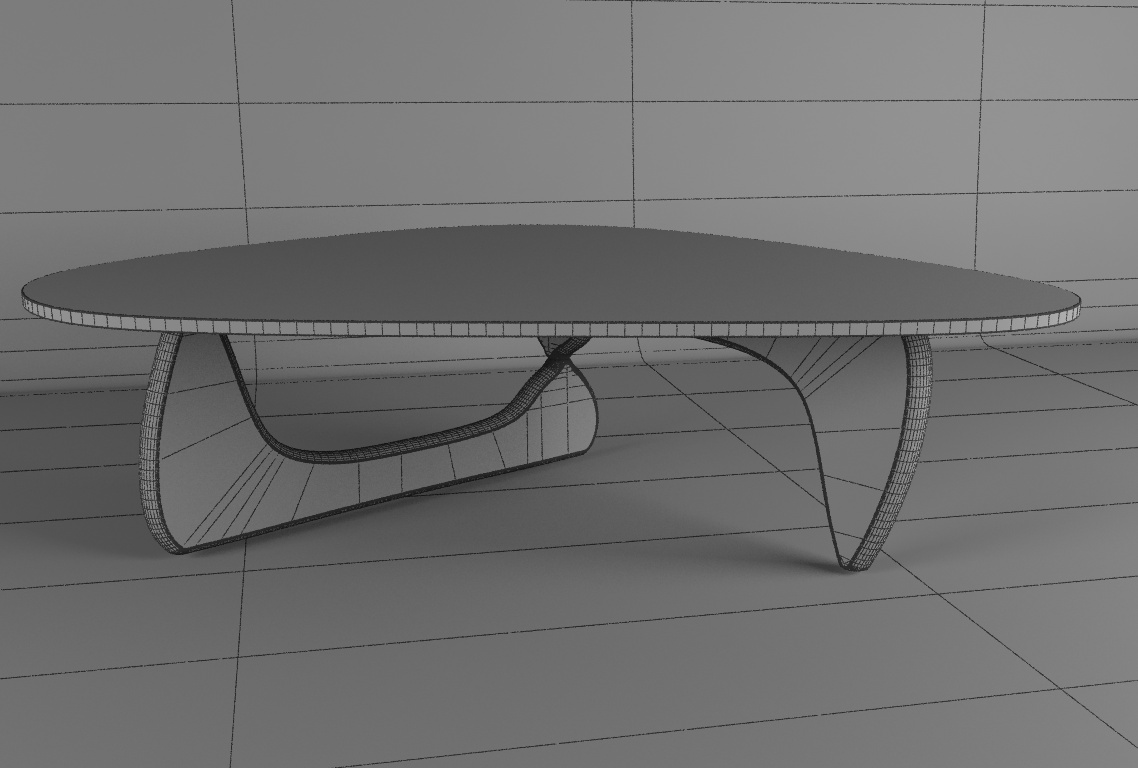
\includegraphics[width=10cm]{img/CoffeTableWireShade.jpg}
		\caption{Mental Ray Render, Shaded Wireframe}
	\label{fig:noguchi-1948}
\end{figure}

\begin{figure}[hb]
	\centering
		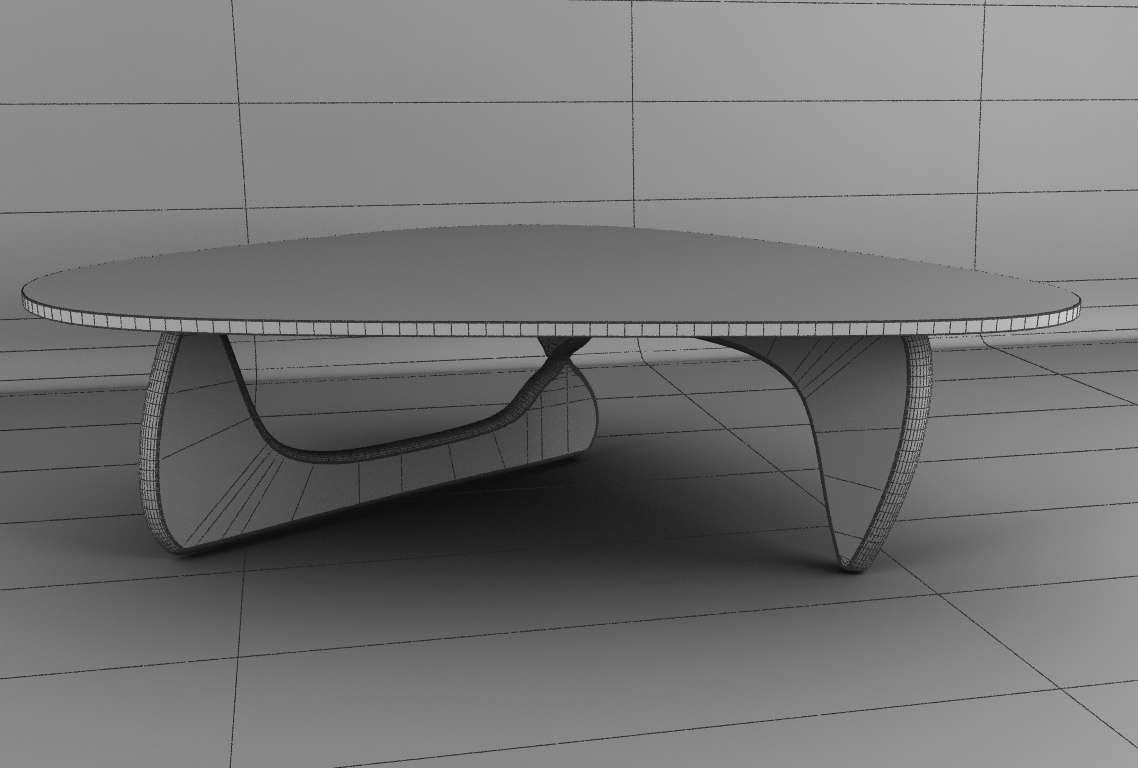
\includegraphics[width=10cm]{img/CoffeTableWireShadeAO.jpg}
		\caption{Mental Ray Shaded Wireframe with Ambient Occlusion}
	\label{fig:noguchi-1948}
\end{figure}

\begin{figure}[hb]
	\centering
		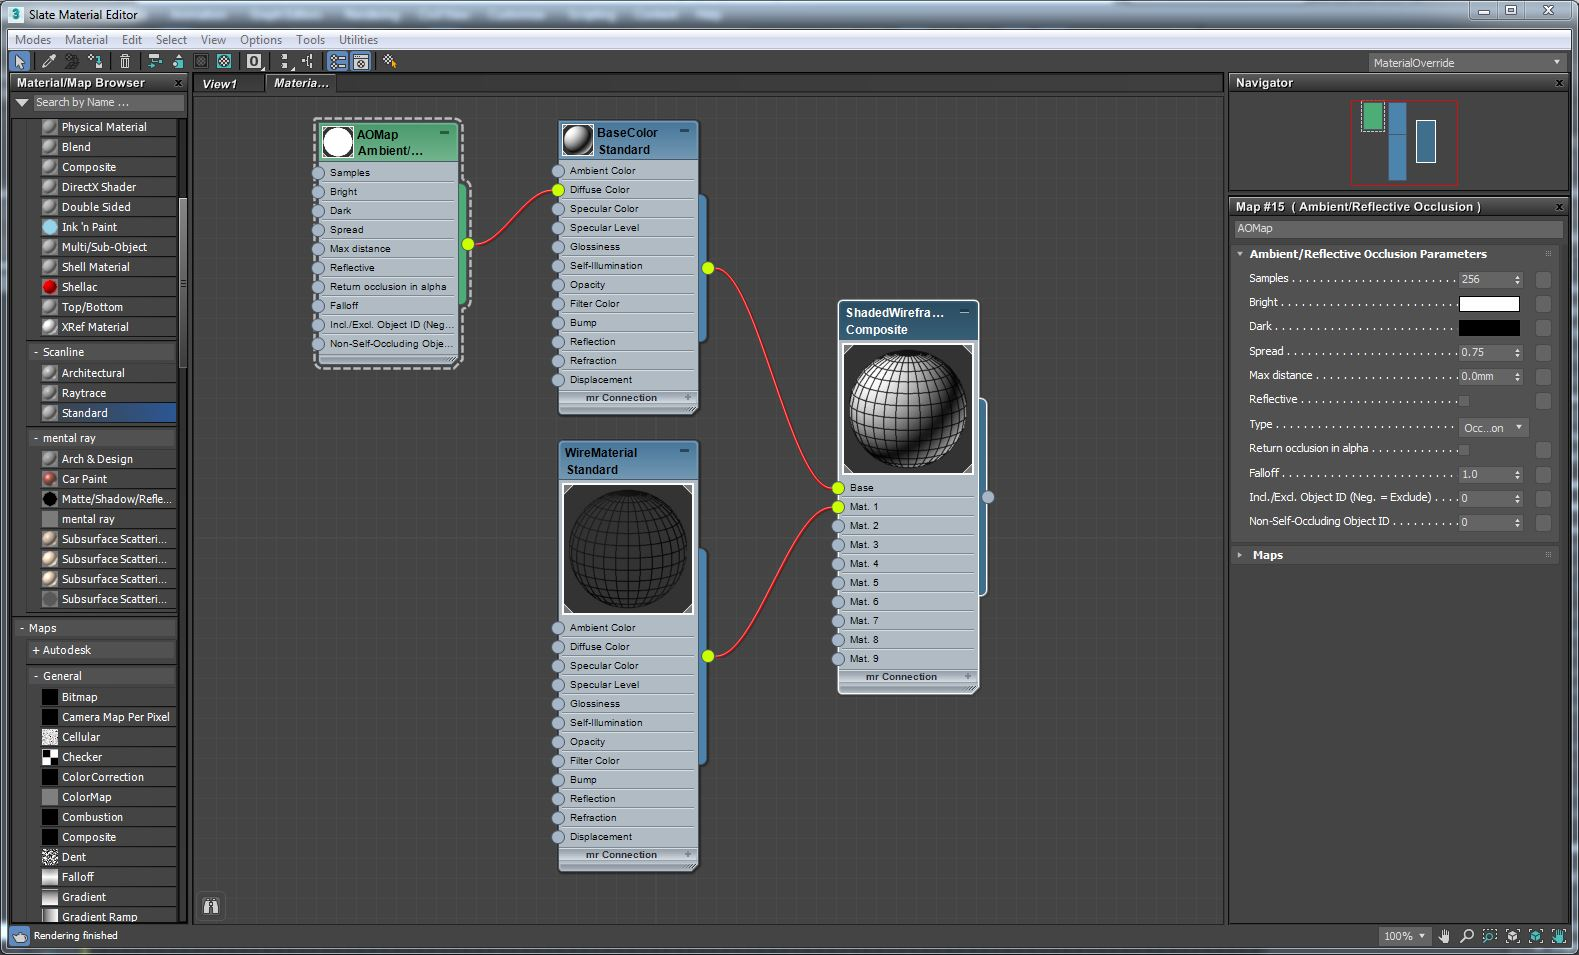
\includegraphics[width=10cm]{img/ShadedWireframeMaterial.jpg}
		\caption{Ambient Occlusion Material}
	\label{fig:noguchi-1948}
\end{figure}




\textbf{How to Structure your Submission}
\\
All submission are to take the form of a single zip file.  The zip file must maintain the folder structure as generated by 3DS Max or Unity.   The images below, figure \ref{fig:3dsstructure} and figure \ref{fig:unity} give an indication of the folder structure that you should zip and submit.\\ \\

\begin{figure}[h]
	\centering
	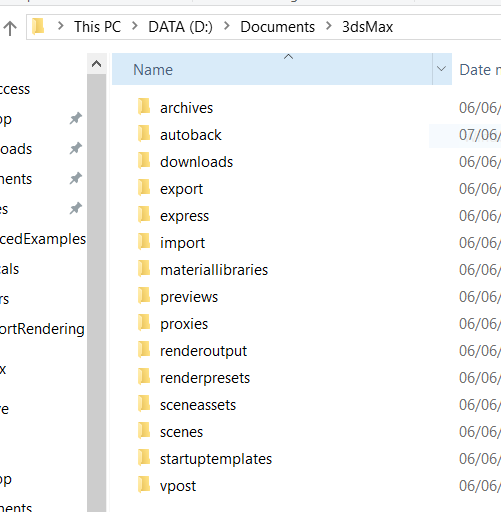
\includegraphics[width=0.5\linewidth]{img/3dsStructure.jpg}
	\caption{3D Studio Max Project Folder Structure}
	\label{fig:3dsstructure}
\end{figure}
\begin{figure}[h]
	\centering
	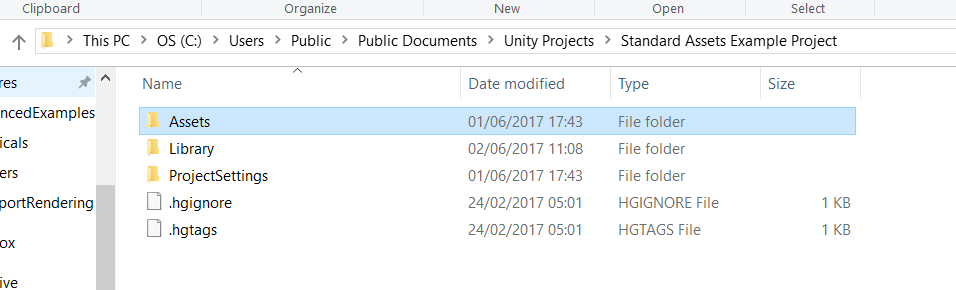
\includegraphics[width=0.9\linewidth]{img/Unity.jpg}
	\caption{Unity Game Engine File Structure}
	\label{fig:unity}
\end{figure}

All assets used during the course of the assignment are to be submitted.  All assets used and created should be placed within the appropriate folder.  To clarify, all 3ds Scene files should be placed within the 'scenes' folder; and all renders should be placed within the 'renderoutput' folder.
\\
\\
Please note that it is not appropriate to submit a single \textit{.max} file, single \textit{.jpg} file, or a single \textit{.unity} file.  

\vspace{1cm}
\textbf{Late Submission}\\
Failure to submit your assignment on or before the date and time indicated on Moodle will result in a penalty of 5\% per day or part thereof.
\\
\\
Late submission penalties will not apply in cases where a valid medical certificate is provided.  In such instances an extension of time will be granted for the duration of illness stated on the medical certificate that falls after the submission date.  A copy of the medical certificate must be included with the late submission.
\\
\\
Late submission penalties may also be avoided in exceptional circumstances.  These will be dealt with on a case by case basis.  Please note that loss of pen-drives, inability to use or access the software etc. will not be considered 'exceptional circumstances'.




\end{document}